\documentclass[ %handout, % for handouts %%% 12pt,handout,
usenames,dvipsnames,
aspectratio=169,11pt]{beamer}

\usepackage[ruled, linesnumbered]{algorithm2e}

\usepackage{tcolorbox}
 \tcbuselibrary{skins,raster}
\usepackage{outlines}
\usepackage{multirow}
\usepackage{babel}
\usepackage{blindtext}
\usepackage{verbatim}
\usepackage{minted}

\usetikzlibrary{decorations.text,arrows.meta,bending}

\newcommand{\verteq}{\rotatebox{90}{$\,=$}}

\usepackage{pgfplots}
\pgfplotsset{compat=1.14}
\usepgfplotslibrary{statistics}

\setbeamertemplate{navigation symbols}{}

 \usepackage{relsize}

\usepackage{bookmark}

%\usepackage[hyperref]{xcolor}


\let\oldcite=\cite
\renewcommand{\cite}[1]{\textcolor[rgb]{.7,.7,.7}{\oldcite{#1}}}



\mode<presentation> {

% The Beamer class comes with a number of default slide themes
% which change the colors and layouts of slides. Below this is a list
% of all the themes, uncomment each in turn to see what they look like.

%\usetheme{default}
%\usetheme{AnnArbor}
%\usetheme{Antibes}
%\usetheme{Bergen}
%\usetheme{Berkeley}
%\usetheme{Berlin}
%\usetheme{Boadilla}
%\usetheme{CambridgeUS}
%\usetheme{Copenhagen}
%\usetheme{Darmstadt}
%\usetheme{Dresden}
%\usetheme{Frankfurt}
%\usetheme{Goettingen}
%\usetheme{Hannover}
%\usetheme{Ilmenau}
%\usetheme{JuanLesPins}
%\usetheme{Luebeck}
\usetheme{Madrid}
%\usetheme{Malmoe}
%\usetheme{Marburg}
%\usetheme{Montpellier}
%\usetheme{PaloAlto}
%\usetheme{Pittsburgh}
%\usetheme{Rochester}
%\usetheme{Singapore}
%\usetheme{Szeged}
%\usetheme{Warsaw}

% As well as themes, the Beamer class has a number of color themes
% for any slide theme. Uncomment each of these in turn to see how it
% changes the colors of your current slide theme.

%\usecolortheme{albatross}
%\usecolortheme{beaver}
%\usecolortheme{beetle}
%\usecolortheme{crane}
%\usecolortheme{dolphin}
%\usecolortheme{dove}
%\usecolortheme{fly}
%\usecolortheme{lily}
%\usecolortheme{orchid}
%\usecolortheme{rose}
%\usecolortheme{seagull}
%\usecolortheme{seahorse}
%\usecolortheme{whale}
%\usecolortheme{wolverine}

%\setbeamertemplate{footline} % To remove the footer line in all slides uncomment this line
%\setbeamertemplate{footline}[page number] % To replace the footer line in all slides with a simple slide count uncomment this line

%\setbeamertemplate{navigation symbols}{} % To remove the navigation symbols from the bottom of all slides uncomment this line
}

\setbeamercolor{itemize item}{fg=white}
%\setbeamercolor{itemize subitem}{fg=blue}
%\setbeamercolor{itemize subsubitem}{fg=cyan}

\setbeamertemplate{itemize item}[circle]
%\setbeamertemplate{itemize subitem}[circle]
%\setbeamertemplate{itemize subsubitem}[triangle]

\setbeamercolor{frametitle}{fg=white}
\setbeamercolor{section in head/foot}{bg=white}
\setbeamercolor{author in head/foot}{bg=white}
\setbeamercolor{date in head/foot}{fg=white}

\setbeamercolor{background canvas}{bg=black}
\setbeamercolor{normal text}{fg=white}

\usepackage[absolute,overlay]{textpos}
\usepackage{graphicx}
\usepackage{booktabs} % Allows the use of \toprule, \midrule and \bottomrule in tables
\usepackage{forest}
 \usepackage{tikz}
 \usetikzlibrary{shapes.geometric}
\usepackage{rotating}
\usepackage[]{wrapfig}
\usetikzlibrary{arrows,shapes}
\usetikzlibrary{trees,matrix}
\usepackage{multirow}
\usepackage{dirtree}
%\usepackage{color, colortbl}
\definecolor{Gray}{gray}{0.85}
\newcommand\x{.11}
\graphicspath{ {Images/} }
\usepackage{mathrsfs}
%\usepackage[symbol]{footmisc}

%\usepackage{xcolor}
%\hypersetup{
%  colorlinks,
%  allcolors=.,
%  urlcolor=ProcessBlue,
%}
%\hypersetup{colorlinks = true,
%%            linkcolor = red,
 %           urlcolor=ProcessBlue,
 %           citecolor = green,
 %           anchorcolor = blue}

%\usepackage{bibunits}
%\setbeamertemplate{bibliography item}{[\theenumiv]}
%\defaultbibliography{IoT,CPS}
%\defaultbibliographystyle{IEEEtran}

\usepackage[numbers]{natbib}
\usepackage{bibunits}

%If by "animated" you mean creating overlays, then a straight application of Daniel's visible on key would solve the problem.
%Step 1. Put the following in the preamble:
\tikzset{
    invisible/.style={opacity=0,text opacity=0},
    visible on/.style={alt=#1{}{invisible}},
    alt/.code args={<#1>#2#3}{%
      \alt<#1>{\pgfkeysalso{#2}}{\pgfkeysalso{#3}} % \pgfkeysalso doesn't change the path
    },
}
\forestset{
  visible on/.style={
    %for children={
      /tikz/visible on={#1},
      edge={/tikz/visible on={#1}}
   % }
  }
}


%\AtBeginSection[]
%
%  \begin{frame}<beamer>
%    \frametitle{Outline}
%    \tableofcontents[currentsection]
%  \end{frame}
%}

%\AtBeginSubsection[]
%{
%  \begin{frame}<beamer>
%    \frametitle{Outline}
%    \tableofcontents[currentsubsection]
% \end{frame}
%}

% \logo{\raisebox{-0.5cm}{\includegraphics[width=1cm]{naulogo.png}}\hspace*{0.5cm}}

\newenvironment{stepitemize}{\begin{itemize}[<+->]}{\end{itemize} }

\newcommand{\myblue}{\only{\color{blue}}}
\newcommand{\mygreen}{\only{\color{green}}}
\newcommand{\myyellow}{\only{\color{yellow}}}
\newcommand{\myorange}{\only{\color{orange}}}
\newcommand{\myred}{\only{\color{red}}}
\newcommand{\Z}{\mathbb{Z}}
\newcommand{\Q}{\mathbb{Q}}
\newcommand{\R}{\mathbb{R}}
\newcommand{\C}{\mathbb{C}}
\newcommand{\RR}{\mbox{\msbm R}}
\newcommand{\F}{\mathbb{F}}
\newcommand{\Rs}{\mathcal{R}}
\newcommand{\Hs}{\mathbb{H}}

\begin{document}

\title[HE]{
HE: An Introduction to What/Why/How}
\author{Bahattin Yildiz}
\institute[DBIO-Glade]{DBIO-Glade}
\date[November]{November 2022}
\maketitle

\section{Acknowledgement}
\begin{frame}{Acknowledgement}
With contributions from
\begin{itemize}
\item Flavio Bergamaschi
\item Hamish Hunt
\item Jack Crawford
\item Tabitha Ogilvie
\end{itemize}

\end{frame}

\section{Introduction}
\begin{frame}\frametitle{Introduction}
\begin{stepitemize}
\item Inaugural lecture
\item Followed by a series of in-depth lectures (HE-Math Lectures)
\item Understand the inner workings of HE
\item Requires a build-up from the Number Theory basics
\item Up to Galois Theory and polynomial rings.
\item Today: ``taste" of what is to come.
\end{stepitemize}
\end{frame}

\section{Why HE?}
\begin{frame} {Standard Cryptography}
\begin{center}
    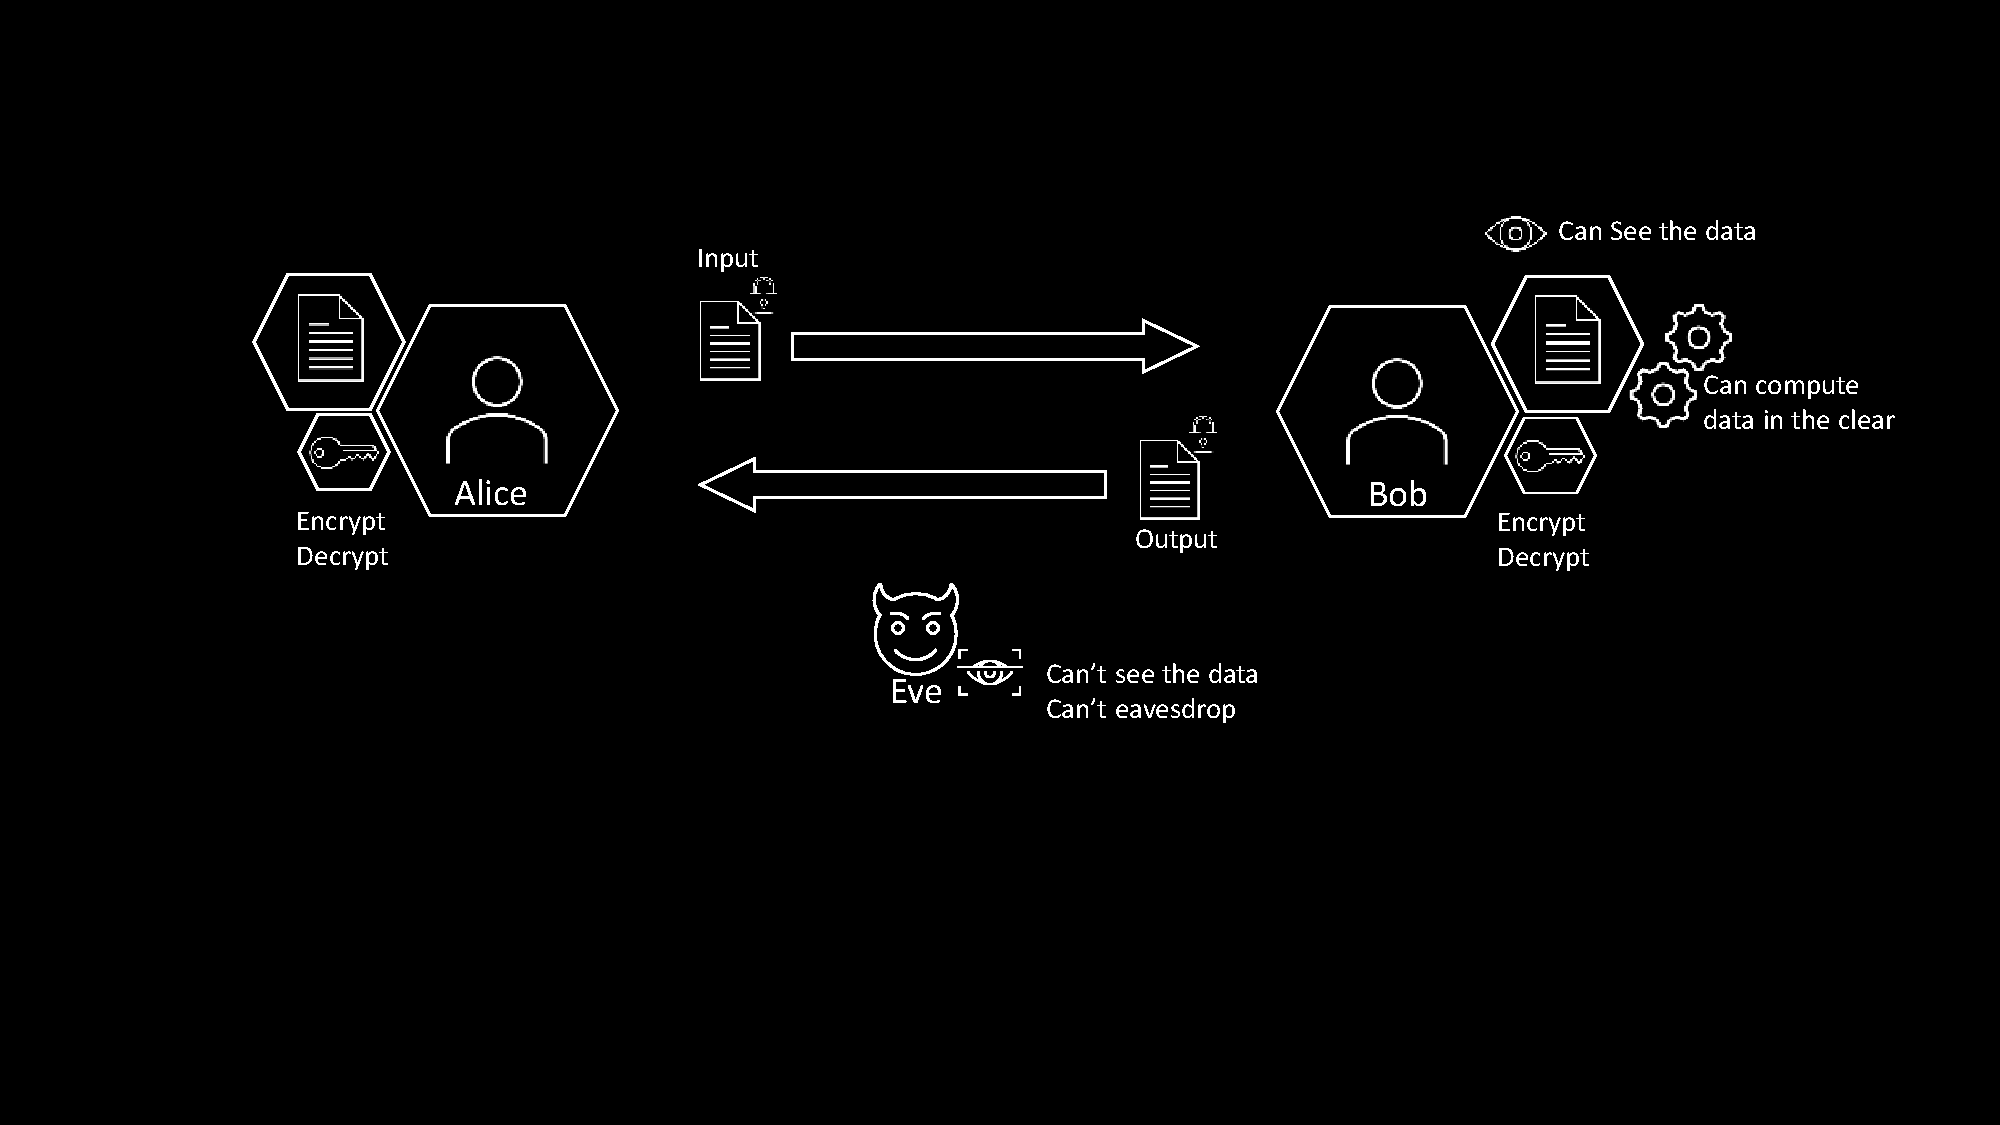
\includegraphics[scale=.38]{images/StandardData.pdf}
\end{center}
\end{frame}

\begin{frame}{Cryptography with Homomorphic Encryption}
\begin{center}
    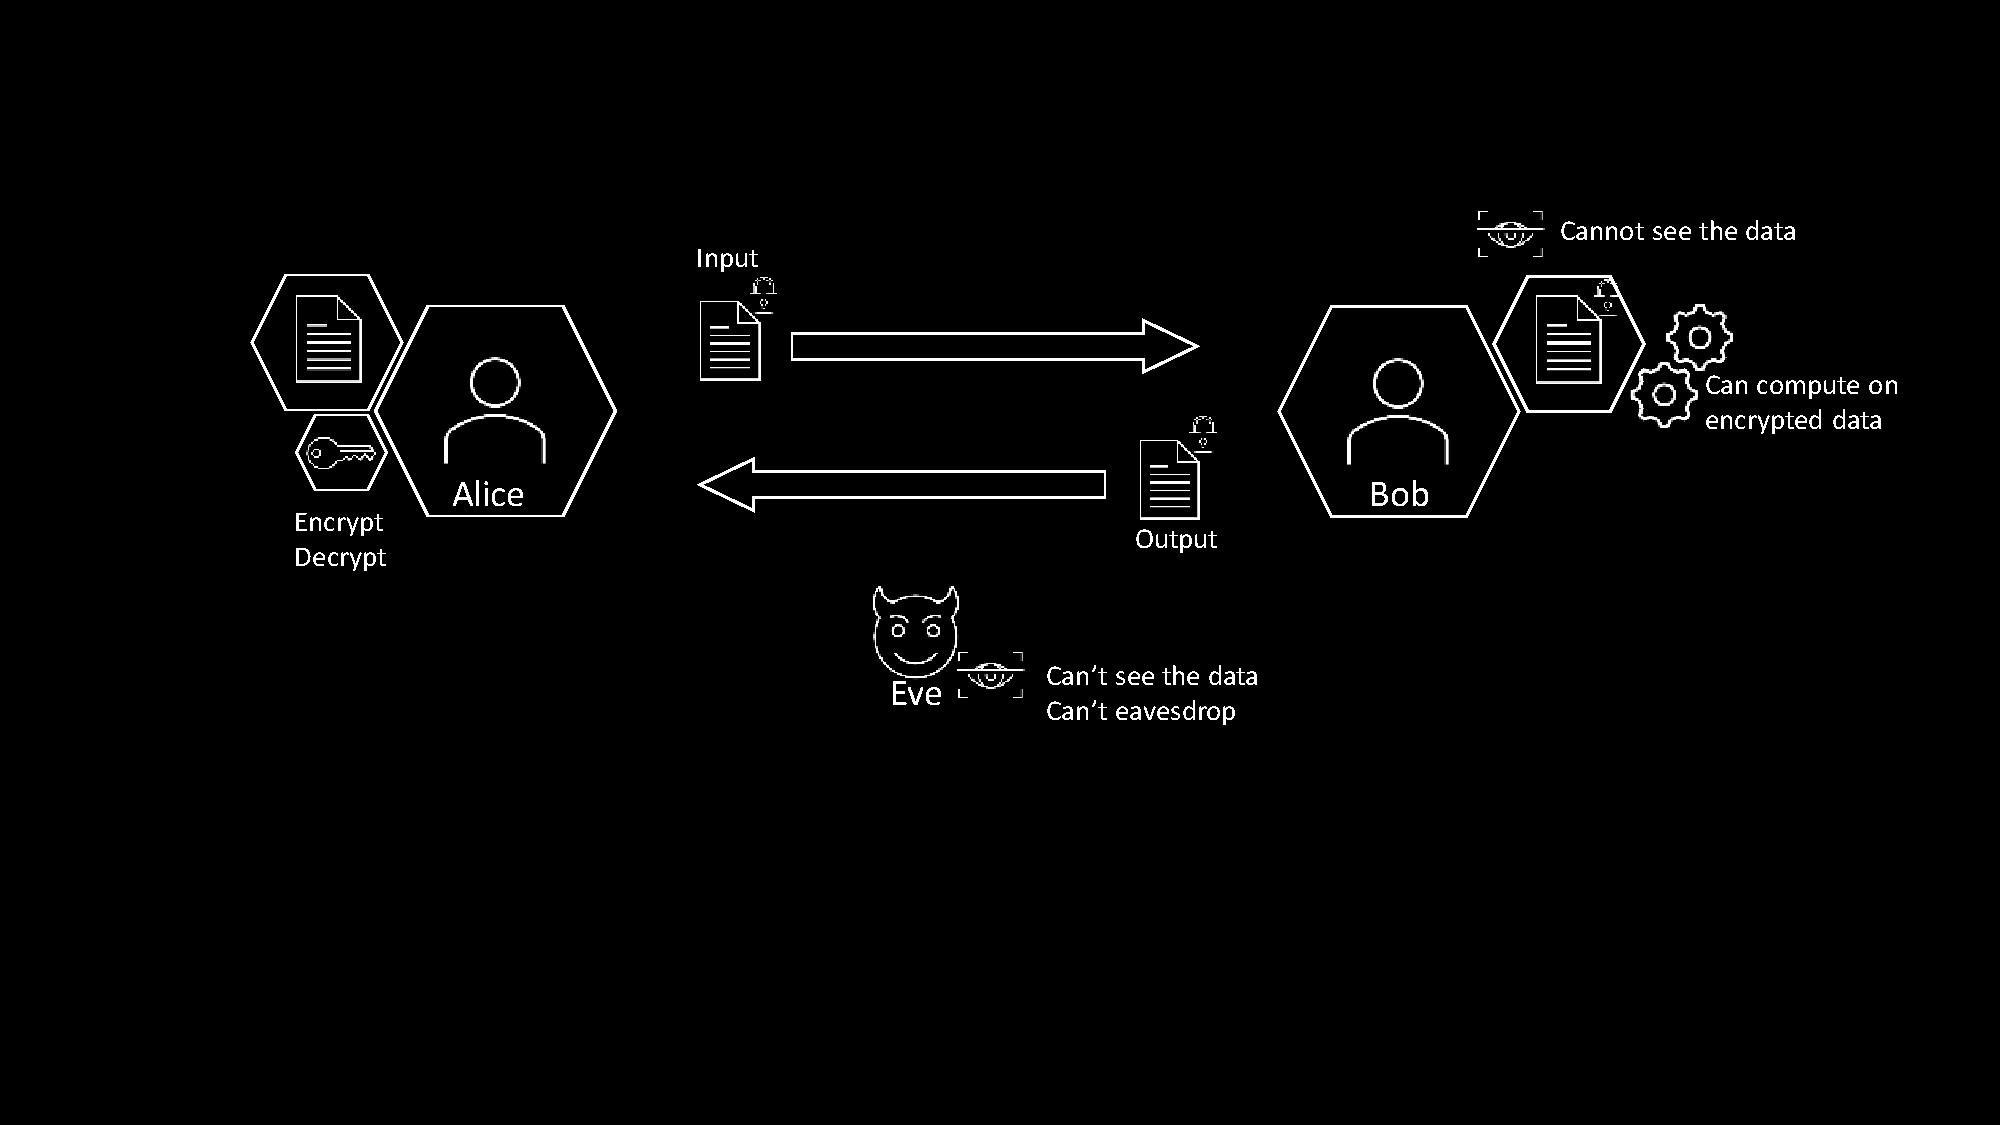
\includegraphics[scale=.38]{images/HomomorphicData.pdf}
\end{center}
\end{frame}

\begin{frame}{Data Status}
\begin{center}
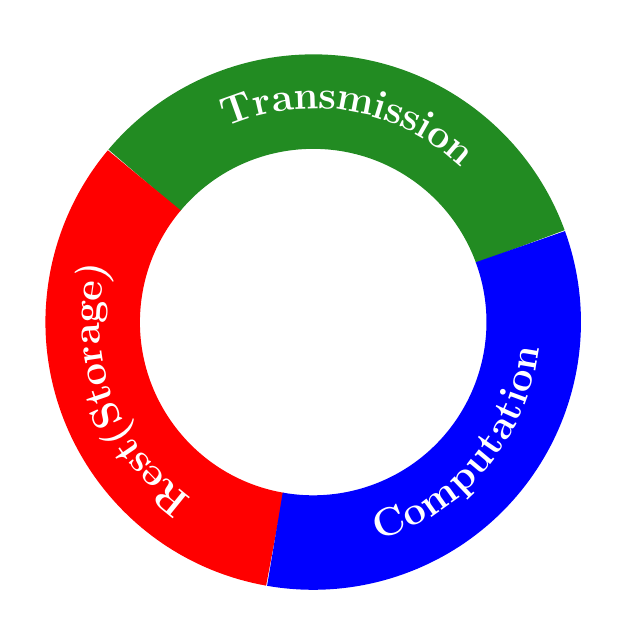
\begin{tikzpicture}
% \tikzset{mytriangle/.tip={Triangle[length = 0pt .95,width=0pt  1.45,round,line width=0pt .1]}}

\newcommand*{\LineWidth}{1.2cm}
    \newcommand*{\Radius}{2.8cm}
    %% Text:
    \node[font=\sffamily,scale=2.5,anchor=south,color=white] at (0,-0.1) {Data};
    \node[font=\sffamily,scale=2.5,anchor=north,color=white] at (0,0.5) {Encrypted};
    %% Arrow shafts:
    \foreach \X [count=\Y] in {ForestGreen,red,blue} {
        \draw[line width=\LineWidth,\X,rotate=120*(\Y-1)]
             (140:\Radius) arc (140:20:\Radius);
    }
    %% Arrowheads
%    \foreach \X [count=\Y] in {gray,red,blue} {
 %       \draw[-mytriangle,line width=\LineWidth,\X,rotate=120*(\Y-1)]
 %            (60:\Radius) arc (60:5:\Radius);
 %   }

 %  \foreach \X [count=\Y] in {gray,red,blue} {
  %      \draw[-mytriangle,line width=\LineWidth,\X,rotate=120*(\Y-1)]
   %          (120:\Radius) arc (120:5:\Radius);
   % }

    %% Text on arrows:
    \foreach \X/\reverse [count=\Y] in {Transmission/true, Rest(Storage)/true,Computation/false} {
        \path[rotate=120*(\Y-1),decorate,decoration={text along path,text={|\Large\bfseries|\X},
                raise=-2.5pt,text color=white,text align=center,reverse path=\reverse}]
             (80-40:\Radius) arc(80-40:80+40:\Radius);

    }
\end{tikzpicture}
\end{center}
\end{frame}


\begin{frame}{New Model}
\begin{stepitemize}
\item Pre-homomorphic Encryption Business Model:

\bigskip
\begin{center}
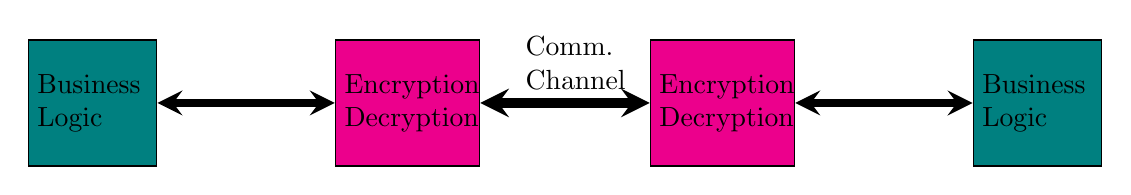
\begin{tikzpicture}

\node[rectangle,draw,  minimum width = 1.6cm,
    minimum height = 1.6cm, fill=teal, text width=1.4 cm] (r1) at (0,0) {Business Logic};

 \node[rectangle,draw,  minimum width = 1.6cm,
    minimum height = 1.6cm, fill=magenta, text width=1.6 cm] (r2) at (4,0) {Encryption Decryption};
 \node[rectangle,draw,  minimum width = 1.6cm,
    minimum height = 1.6cm, fill=magenta, text width=1.6 cm] (r3) at (8,0) {Encryption Decryption};
\node[rectangle,draw,  minimum width = 1.6cm,
    minimum height = 1.6cm, fill=teal, text width=1.4 cm] (r4) at (12,0) {Business Logic};
\draw[stealth-stealth, line width=1mm] (r1)--(r2);
\draw[stealth-stealth, line width=1.2mm] (r2)--node [above, text width=1 cm] {Comm. Channel} (r3);
\draw[stealth-stealth, line width=1mm] (r3)--(r4);
\end{tikzpicture}
\end{center}

\bigskip

\item Post-homomorphic Encryption Business Model:

\bigskip
\begin{center}
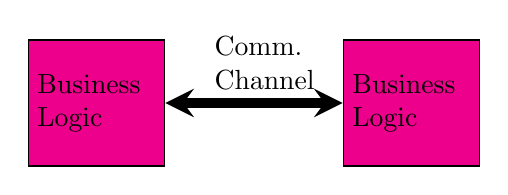
\begin{tikzpicture}
 \node[rectangle,draw, fill=magenta, minimum width = 1.6cm,
    minimum height = 1.6cm, text width=1.5 cm] (q1) at (4,-4) {Business Logic};
 \node[rectangle,draw, fill=magenta, minimum width = 1.6cm,
    minimum height = 1.6cm, text width=1.5 cm] (q2) at (8,-4) {Business Logic};
\draw[stealth-stealth, line width=1.2mm] (q1)--node [above, text width=1 cm] {Comm. Channel} (q2);
\end{tikzpicture}
\end{center}
\end{stepitemize}
\end{frame}

\begin{frame}{The New Paradigm: Inter- and intra-organization collaboration}
    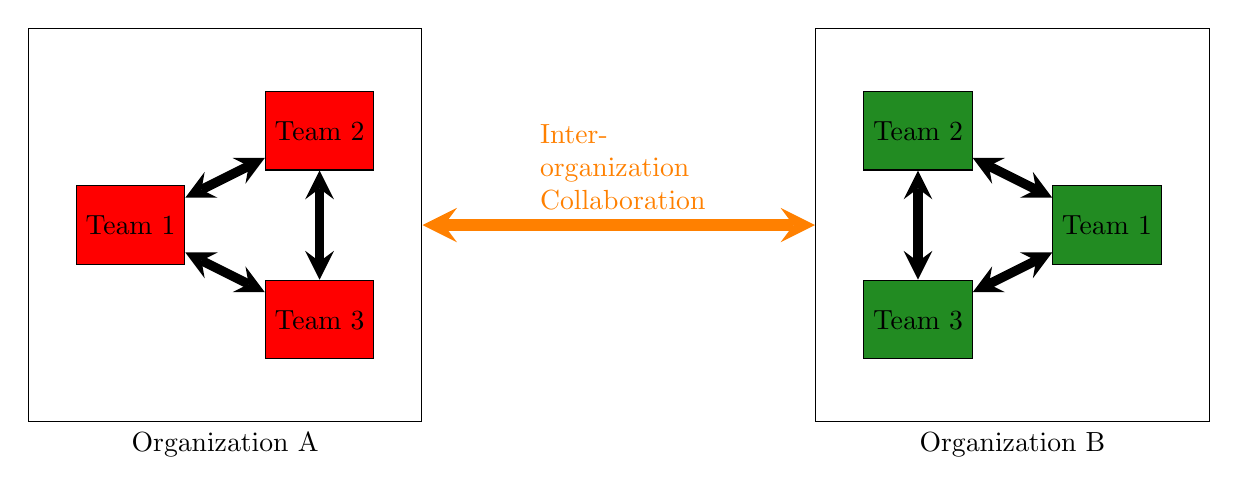
\begin{tikzpicture}
    \node[rectangle,draw, fill=white, minimum width = 5cm,
    minimum height = 5cm] (q1) at (0,0){};
    \node[rectangle,draw, fill=white, minimum width = 5cm,
    minimum height = 5cm] (q2) at (10,0){};
    \node [below] (P1) at (q1.south) {Organization A};
    \node [below] (P2) at (q2.south) {Organization B};
    \node[rectangle,draw, fill=red, minimum width = 1cm,
    minimum height = 1cm] (r1) at (-1.2,0){Team 1};
    \node[rectangle,draw, fill=red, minimum width = 1cm,
    minimum height = 1cm] (r2) at (1.2,1.2){Team 2};
    \node[rectangle,draw, fill=red, minimum width = 1cm,
    minimum height = 1cm] (r3) at (1.2,-1.2){Team 3};

    \node[rectangle,draw, fill=ForestGreen, minimum width = 1cm,
    minimum height = 1cm] (s1) at (11.2,0){Team 1};
    \node[rectangle,draw, fill=ForestGreen, minimum width = 1cm,
    minimum height = 1cm] (s2) at (8.8,1.2){Team 2};
    \node[rectangle,draw, fill=ForestGreen, minimum width = 1cm,
    minimum height = 1cm] (s3) at (8.8,-1.2){Team 3};

    \draw[stealth-stealth, color=black, line width=1.2mm] (s2)--(s3);
    \draw[stealth-stealth, color=black, line width=1.2mm] (s1)--(s2);
    \draw[stealth-stealth, color=black, line width=1.2mm] (s1)--(s3);


    \draw[stealth-stealth, color=black, line width=1.2mm] (r2)--(r3);
    \draw[stealth-stealth, color=black, line width=1.2mm] (r1)--(r2);
    \draw[stealth-stealth, color=black, line width=1.2mm] (r1)--(r3);
    \draw[stealth-stealth, color=orange, line width=1.5mm] (q1)--node [above, text width=2 cm] {Inter-organization Collaboration}(q2);
 \end{tikzpicture}
\end{frame}

\begin{frame}{Trust vs Collaboration}
\begin{stepitemize}
\item Need-to-know vs need-to-share.
\item Insourcing-outsourcing
\end{stepitemize}
\end{frame}

\section{Basic Mathematical Tools}
\begin{frame}{Start with sets}
    \begin{stepitemize}
    \item $\Z=\{\dots, -2,-1,0,1,2,\dots \}$: Set of integers
    \item $\R$: Set of real numbers
    \item $\Z_q$: Set of residue classes modulo $q$
    \item $\Z_q=\{0,1,\dots,q-1\}$.
    \item $\Z[x]$: Set of polynomials with integer coefficients.
    \item $\Z[x]=\{a_0+a_1x+\dots +a_nx^n| \: n\geq 0, a_i\in \Z\}.$
    \end{stepitemize}
\end{frame}

\begin{frame}{Operations}
\begin{stepitemize}
    \item  $\Z_5=\{0,1,2,3,4\}$
    \item We can add and multiply modulo 5
    \item Different properties with each operation
    \item Operation tables:
\end{stepitemize}
\end{frame}

\begin{frame}{Operation Tables}
\begin{itemize}
\item[]<1-> \only<1>{     \begin{table}
            \begin{tabular}{ c| c | c |c|c|c}
$\oplus$  & $0$ & $1$ & $2$ & $3$& $4$\\
\hline
$0$ & $0$ & $1$ & $2$ & $3$& $4$ \\
\hline
$1$ & $1$ & $2$ & $3$ & $4$ & $0$ \\
\hline
$2$& $2$ & $3$ &$4$ & $0$ & $1$\\
\hline
$3$& $3$ & $4$ &$0$ & $1$ & $2$\\
\hline
$4$& $4$ & $0$ & $1$ & $2$ & $3$
\end{tabular}
\caption{Addition table for $\Z_5$}
\end{table}
}\only<2>{   \begin{table}
            \begin{tabular}{ c| c | c |c|c|c}
$\oplus$  & {\color{blue}$0$} & $1$ & $2$ & $3$& $4$\\
\hline
{\color{blue} $0$} & {\color{blue}$0$} & {\color{blue} $1$} & {\color{blue}$2$} & {\color{blue}$3$}& {\color{blue} $4$} \\
\hline
$1$ & {\color{blue}$1$} & $2$ & $3$ & $4$ & {$0$} \\
\hline
$2$& {\color{blue}$2$} & $3$ &$4$ & $0$ & $1$\\
\hline
$3$& {\color{blue}$3$} & $4$ &$0$ & $1$ & $2$\\
\hline
$4$& {\color{blue}$4$} & $0$ & $1$ & $2$ & $3$
\end{tabular}
\caption{Addition table for $\Z_5$}
\end{table}
}
\only<3>{\begin{table}
            \begin{tabular}{ c| c | c |c|c|c}
$\oplus$  & {\color{blue}$0$} & $1$ & $2$ & $3$& $4$\\
\hline
{\color{blue} $0$} & {\color{blue}$0$} & {\color{blue} $1$} & {\color{blue}$2$} & {\color{blue}$3$}& {\color{blue} $4$} \\
\hline
$1$ & {\color{blue}$1$} & $2$ & $3$ & $4$ & {\color{red}$0$} \\
\hline
$2$& {\color{blue}$2$} & $3$ &$4$ & {\color{red}$0$} & $1$\\
\hline
$3$& {\color{blue}$3$} & $4$ &{\color{red}$0$} & $1$ & $2$\\
\hline
$4$& {\color{blue}$4$} & {\color{red}$0$} & $1$ & $2$ & $3$
\end{tabular}
\caption{Addition table for $\Z_5$}
\end{table}
}
\only<4>{
\begin{columns}
\begin{column}{0.4\textwidth}
\begin{table}
            \begin{tabular}{ c| c | c |c|c|c}
$\oplus$  & {\color{blue}$0$} & $1$ & $2$ & $3$ & $4$\\
\hline
{\color{blue} $0$} & {\color{blue}$0$} & {\color{blue} $1$} & {\color{blue}$2$} & {\color{blue}$3$}& {\color{blue} $4$} \\
\hline
$1$ & {\color{blue}$1$} & $2$ & $3$ & $4$ & {\color{red}$0$} \\
\hline
$2$& {\color{blue}$2$} & $3$ &$4$ & {\color{red}$0$} & $1$\\
\hline
$3$& {\color{blue}$3$} & $4$ &{\color{red}$0$} & $1$ & $2$\\
\hline
$4$& {\color{blue}$4$} & {\color{red}$0$} & $1$ & $2$ & $3$
\end{tabular}
\caption{Addition table for $\Z_5$}
\end{table}
    \end{column}

        \begin{column}{0.4\textwidth}
    \begin{table}
            \begin{tabular}{ c| c | c |c|c|c}
$\odot$  & $0$ & $1$ & $2$ & $3$& $4$\\
\hline
$0$ & $0$ & $0$ & $0$ & $0$& $0$ \\
\hline
$1$ & $0$ & $1$ & $2$ & $3$ & $4$ \\
\hline
$2$& $0$ & $2$ &$4$ & $1$ & $3$\\
\hline
$3$& $0$ & $3$ &$1$ & $4$ & $2$\\
\hline
$4$& $0$ & $4$ & $3$ & $2$ & $1$
\end{tabular}
\caption{Multiplication table for $\Z_5$}
\end{table}
    \end{column}
\end{columns}
}
\only<5>{
\begin{columns}
\begin{column}{0.4\textwidth}
\begin{table}
            \begin{tabular}{ c| c | c |c|c|c}
$\oplus$  & {\color{blue}$0$} & $1$ & $2$ & $3$& $4$\\
\hline
{\color{blue} $0$} & {\color{blue}$0$} & {\color{blue} $1$} & {\color{blue}$2$} & {\color{blue}$3$}& {\color{blue} $4$} \\
\hline
$1$ & {\color{blue}$1$} & $2$ & $3$ & $4$ & {\color{red}$0$} \\
\hline
$2$& {\color{blue}$2$} & $3$ &$4$ & {\color{red}$0$} & $1$\\
\hline
$3$& {\color{blue}$3$} & $4$ &{\color{red}$0$} & $1$ & $2$\\
\hline
$4$& {\color{blue}$4$} & {\color{red}$0$} & $1$ & $2$ & $3$
\end{tabular}
\caption{Addition table for $\Z_5$}
\end{table}
    \end{column}

        \begin{column}{0.4\textwidth}
    \begin{table}
            \begin{tabular}{ c| c | c |c|c|c}
$\odot$  & $0$ & {\color{blue}$1$} & $2$ & $3$& $4$\\
\hline
$0$ & $0$ & {\color{blue}$0$} & $0$ & $0$& $0$ \\
\hline
{\color{blue} $1$} & {\color{blue}$0$} & {\color{blue}$1$} & {\color{blue}$2$} & {\color{blue}$3$} & {\color{blue}$4$} \\
\hline
$2$& $0$ & {\color{blue}$2$} &$4$ & $1$ & $3$\\
\hline
$3$& $0$ & {\color{blue}$3$} &$1$ & $4$ & $2$\\
\hline
$4$& $0$ & {\color{blue}$4$} & $3$ & $2$ & $1$
\end{tabular}
\caption{Multiplication table for $\Z_5$}
\end{table}
    \end{column}
\end{columns}
}
\only<6>{
\begin{columns}
\begin{column}{0.4\textwidth}
\begin{table}
            \begin{tabular}{ c| c | c |c|c|c}
$\oplus$  & {\color{blue}$0$} & $1$ & $2$ & $3$& $4$\\
\hline
{\color{blue} $0$} & {\color{blue}$0$} & {\color{blue} $1$} & {\color{blue}$2$} & {\color{blue}$3$}& {\color{blue} $4$} \\
\hline
$1$ & {\color{blue}$1$} & $2$ & $3$ & $4$ & {\color{red}$0$} \\
\hline
$2$& {\color{blue}$2$} & $3$ &$4$ & {\color{red}$0$} & $1$\\
\hline
$3$& {\color{blue}$3$} & $4$ &{\color{red}$0$} & $1$ & $2$\\
\hline
$4$& {\color{blue}$4$} & {\color{red}$0$} & $1$ & $2$ & $3$
\end{tabular}
\caption{Addition table for $\Z_5$}
\end{table}
    \end{column}

        \begin{column}{0.4\textwidth}
    \begin{table}
            \begin{tabular}{ c| c | c |c|c|c}
$\odot$  & $0$ & {\color{red}$1$} & {\color{red} $2$} & {\color{red}$3$}& {\color{red}$4$}\\
\hline
$0$ & $0$ & $0$ & $0$ & $0$& $0$ \\
\hline
{\color{red} $1$} & $0$ & {\color{red}$1$} & {\color{red}$2$} & {\color{red}$3$} & {\color{red}$4$} \\
\hline
{\color{red}$2$}& $0$ & {\color{red}$2$} &{\color{red}$4$} & {\color{red}$1$} & {\color{red} $3$}\\
\hline
{\color{red} $3$}& $0$ & {\color{red}$3$} &{\color{red}$1$} & {\color{red}$4$} & {\color{red}$2$}\\
\hline
{\color{red}$4$}& $0$ & {\color{red}$4$} & {\color{red}$3$} & {\color{red}$2$} & {\color{red}$1$}
\end{tabular}
\caption{Multiplication table for $\Z_5$}
\end{table}
    \end{column}
\end{columns}
}
\only<7>{
\begin{columns}
\begin{column}{0.4\textwidth}
\begin{table}
            \begin{tabular}{ c| c | c |c|c|c}
$\oplus$  & {\color{blue}$0$} & $1$ & $2$ & $3$& $4$\\
\hline
{\color{blue} $0$} & {\color{blue}$0$} & {\color{blue} $1$} & {\color{blue}$2$} & {\color{blue}$3$}& {\color{blue} $4$} \\
\hline
$1$ & {\color{blue}$1$} & $2$ & $3$ & $4$ & {\color{red}$0$} \\
\hline
$2$& {\color{blue}$2$} & $3$ &$4$ & {\color{red}$0$} & $1$\\
\hline
$3$& {\color{blue}$3$} & $4$ &{\color{red}$0$} & $1$ & $2$\\
\hline
$4$& {\color{blue}$4$} & {\color{red}$0$} & $1$ & $2$ & $3$
\end{tabular}
\caption{Addition table for $\Z_5$}
\end{table}
    \end{column}

        \begin{column}{0.4\textwidth}
    \begin{table}
            \begin{tabular}{ c| c | c |c|c|c}
$\odot$  & $0$ & {\color{red}$1$} & {\color{red} $2$} & {\color{red}$3$}& {\color{red}$4$}\\
\hline
$0$ & $0$ & $0$ & $0$ & $0$& $0$ \\
\hline
{\color{red} $1$} & $0$ & {\color{red}$1$} & {\color{red}$2$} & {\color{red}$3$} & {\color{red}$4$} \\
\hline
{\color{red}$2$}& $0$ & {\color{red}$2$} &{\color{red}$4$} & {\color{red}$1$} & {\color{red} $3$}\\
\hline
{\color{red} $3$}& $0$ & {\color{red}$3$} &{\color{red}$1$} & {\color{red}$4$} & {\color{red}$2$}\\
\hline
{\color{red}$4$}& $0$ & {\color{red}$4$} & {\color{red}$3$} & {\color{red}$2$} & {\color{red}$1$}
\end{tabular}
\caption{Multiplication table for $\Z_5$}
\end{table}
    \end{column}
\end{columns}
\bigskip
 \item $(\Z_5,\oplus)$ called a ``group", with $0 \rightarrow$ identity.
   }

\only<8>{
\begin{columns}
\begin{column}{0.4\textwidth}
\begin{table}
            \begin{tabular}{ c| c | c |c|c|c}
$\oplus$  & {\color{blue}$0$} & $1$ & $2$ & $3$& $4$\\
\hline
{\color{blue} $0$} & {\color{blue}$0$} & {\color{blue} $1$} & {\color{blue}$2$} & {\color{blue}$3$}& {\color{blue} $4$} \\
\hline
$1$ & {\color{blue}$1$} & $2$ & $3$ & $4$ & {\color{red}$0$} \\
\hline
$2$& {\color{blue}$2$} & $3$ &$4$ & {\color{red}$0$} & $1$\\
\hline
$3$& {\color{blue}$3$} & $4$ &{\color{red}$0$} & $1$ & $2$\\
\hline
$4$& {\color{blue}$4$} & {\color{red}$0$} & $1$ & $2$ & $3$
\end{tabular}
\caption{Addition table for $\Z_5$}
\end{table}
    \end{column}

        \begin{column}{0.4\textwidth}
    \begin{table}
            \begin{tabular}{ c| c | c |c|c|c}
$\odot$  & $0$ & {\color{red}$1$} & {\color{red} $2$} & {\color{red}$3$}& {\color{red}$4$}\\
\hline
$0$ & $0$ & $0$ & $0$ & $0$& $0$ \\
\hline
{\color{red} $1$} & $0$ & {\color{red}$1$} & {\color{red}$2$} & {\color{red}$3$} & {\color{red}$4$} \\
\hline
{\color{red}$2$}& $0$ & {\color{red}$2$} &{\color{red}$4$} & {\color{red}$1$} & {\color{red} $3$}\\
\hline
{\color{red} $3$}& $0$ & {\color{red}$3$} &{\color{red}$1$} & {\color{red}$4$} & {\color{red}$2$}\\
\hline
{\color{red}$4$}& $0$ & {\color{red}$4$} & {\color{red}$3$} & {\color{red}$2$} & {\color{red}$1$}
\end{tabular}
\caption{Multiplication table for $\Z_5$}
\end{table}
    \end{column}
\end{columns}
\bigskip
 \item $(\Z_5,\oplus)$ called a ``group", with $0 \rightarrow$ identity.
   \item $(\Z_5, \oplus, \odot)$ called a ``ring"
   }

\only<9>{
\begin{columns}
\begin{column}{0.4\textwidth}
\begin{table}
            \begin{tabular}{ c| c | c |c|c|c}
$\oplus$  & {\color{blue}$0$} & $1$ & $2$ & $3$& $4$\\
\hline
{\color{blue} $0$} & {\color{blue}$0$} & {\color{blue} $1$} & {\color{blue}$2$} & {\color{blue}$3$}& {\color{blue} $4$} \\
\hline
$1$ & {\color{blue}$1$} & $2$ & $3$ & $4$ & {\color{red}$0$} \\
\hline
$2$& {\color{blue}$2$} & $3$ &$4$ & {\color{red}$0$} & $1$\\
\hline
$3$& {\color{blue}$3$} & $4$ &{\color{red}$0$} & $1$ & $2$\\
\hline
$4$& {\color{blue}$4$} & {\color{red}$0$} & $1$ & $2$ & $3$
\end{tabular}
\caption{Addition table for $\Z_5$}
\end{table}
    \end{column}

        \begin{column}{0.4\textwidth}
    \begin{table}
            \begin{tabular}{ c| c | c |c|c|c}
$\odot$  & $0$ & {\color{red}$1$} & {\color{red} $2$} & {\color{red}$3$}& {\color{red}$4$}\\
\hline
$0$ & $0$ & $0$ & $0$ & $0$& $0$ \\
\hline
{\color{red} $1$} & $0$ & {\color{red}$1$} & {\color{red}$2$} & {\color{red}$3$} & {\color{red}$4$} \\
\hline
{\color{red}$2$}& $0$ & {\color{red}$2$} &{\color{red}$4$} & {\color{red}$1$} & {\color{red} $3$}\\
\hline
{\color{red} $3$}& $0$ & {\color{red}$3$} &{\color{red}$1$} & {\color{red}$4$} & {\color{red}$2$}\\
\hline
{\color{red}$4$}& $0$ & {\color{red}$4$} & {\color{red}$3$} & {\color{red}$2$} & {\color{red}$1$}
\end{tabular}
\caption{Multiplication table for $\Z_5$}
\end{table}
    \end{column}
\end{columns}
\bigskip
 \item $(\Z_5,\oplus)$ called a ``group", with $0 \rightarrow$ identity.
   \item $(\Z_5, \oplus, \odot)$ called a ``ring"
   \item $0 \rightarrow$ additive identity, while $1\rightarrow$ multiplicative identity
    }

\only<10>{
\begin{columns}
\begin{column}{0.4\textwidth}
\begin{table}
            \begin{tabular}{ c| c | c |c|c|c}
$\oplus$  & {\color{blue}$0$} & $1$ & $2$ & $3$& $4$\\
\hline
{\color{blue} $0$} & {\color{blue}$0$} & {\color{blue} $1$} & {\color{blue}$2$} & {\color{blue}$3$}& {\color{blue} $4$} \\
\hline
$1$ & {\color{blue}$1$} & $2$ & $3$ & $4$ & {\color{red}$0$} \\
\hline
$2$& {\color{blue}$2$} & $3$ &$4$ & {\color{red}$0$} & $1$\\
\hline
$3$& {\color{blue}$3$} & $4$ &{\color{red}$0$} & $1$ & $2$\\
\hline
$4$& {\color{blue}$4$} & {\color{red}$0$} & $1$ & $2$ & $3$
\end{tabular}
\caption{Addition table for $\Z_5$}
\end{table}
    \end{column}

        \begin{column}{0.4\textwidth}
    \begin{table}
            \begin{tabular}{ c| c | c |c|c|c}
$\odot$  & $0$ & {\color{red}$1$} & {\color{red} $2$} & {\color{red}$3$}& {\color{red}$4$}\\
\hline
$0$ & $0$ & $0$ & $0$ & $0$& $0$ \\
\hline
{\color{red} $1$} & $0$ & {\color{red}$1$} & {\color{red}$2$} & {\color{red}$3$} & {\color{red}$4$} \\
\hline
{\color{red}$2$}& $0$ & {\color{red}$2$} &{\color{red}$4$} & {\color{red}$1$} & {\color{red} $3$}\\
\hline
{\color{red} $3$}& $0$ & {\color{red}$3$} &{\color{red}$1$} & {\color{red}$4$} & {\color{red}$2$}\\
\hline
{\color{red}$4$}& $0$ & {\color{red}$4$} & {\color{red}$3$} & {\color{red}$2$} & {\color{red}$1$}
\end{tabular}
\caption{Multiplication table for $\Z_5$}
\end{table}
    \end{column}
\end{columns}
\bigskip
 \item $(\Z_5,\oplus)$ called a ``group", with $0 \rightarrow$ identity.
   \item $(\Z_5, \oplus, \odot)$ called a ``ring"
   \item $0 \rightarrow$ additive identity, while $1\rightarrow$ multiplicative identity
    \item Since $(\{1,2,3,4\},\odot)$ is a group, $\Z_5$ also called a ``field".

  }

\end{itemize}

\end{frame}

\begin{frame}{Can we do the same for polynomials?}
    \begin{stepitemize}
    \item Recall $\Z[x]$ set of polynomials with integer coefficients.
    \item Polynomials in $\Z[x]$ modulo $x^2+1$?
    \item Such polynomials form $\Z[x]/(x^2+1)$.
    \item First, $x^2+1=0 \pmod{x^2+1}$
    \item So $x^2=-1 \pmod{x^2+1}$
    \item So what would $x^3+x^2+2x+1$ be?
    \item Replace $x^2$ by $-1$ and so $x^3$ by $-x$, get $x^3+x^2+2x+1 = x \pmod{x^2+1}$.
    \item Think ``long division".
    \item It is clear that
    $\Z[x]/(x^2+1) = \{ax+b|a, b\in \Z\}$
    \end{stepitemize}
\end{frame}

\begin{frame}{Operations on $\R[x]/(x^2+1)$}
    \begin{stepitemize}
\item Similarly $\R[x]/(x^2+1) = \{ax+b| a,b\in \R\}$.
\item First, $(ax+b)+(cx+d)={\color{cyan}(a+c)x+(b+d)}$
    \item Next,
    $$(ax+b)(cx+d) = acx^2+adx+bcx+bd = {\color{magenta}(ad+bc)x+(bd-ac)}.$$
    \item Looks familiar?
    \item If $ai+b$ and $ci+d$ are complex numbers then
    $$(ai+b)+(ci+d) = {\color{cyan}(a+c)i+(b+d)}$$
    and
   $$ (ai+b)(ci+d) = {\color{magenta}(ad+bc)i+(bd-ac)}.$$
\item This shows $\C \simeq \R[x]/(x^2+1)$.
    \end{stepitemize}
\end{frame}

\begin{frame}{Rings in HE}
\begin{stepitemize}
\item Recall the ring $\Z_p=\{0,1,2, \dots, p-1\}$.
    \item Most operations in some of the HE schemes(such as BGV, BFV) happen in rings $\Z_p[x]/(f(x))$.
    \item Here is the addition and multiplication table of $\Z_2[x]/(x^2+1)$.
    \item Has $4$ elements ($ax+b$, with $a,b=0$ or $1$.)

    \bigskip
    \item []
    \bigskip

    \begin{columns}
        \begin{column}{0.5\textwidth}
     \begin{table}
            \begin{tabular}{ c| c | c |c|c}
$\oplus$  & $0$ & $1$ & $x$ & $1+x$\\
\hline
$0$ & $0$ & $1$ & $x$ & $1+x$ \\
\hline
$1$ & $1$ & $0$ & $1+x$ & $x$ \\
\hline
$x$& $x$ & $1+x$ &$0$ & $1$\\
\hline
$1+x$& $1+x$ & $x$ &$1$ & $0$
\end{tabular}
\end{table}
    \end{column}

        \begin{column}{0.4\textwidth}
    \begin{table}
            \begin{tabular}{ c| c | c |c|c}
$\odot$  & $0$ & $1$ & $x$ & $1+x$\\
\hline
$0$ & $0$ & $0$ & $0$ & $0$ \\
\hline
$1$ & $0$ & $1$ & $x$ & $1+x$ \\
\hline
$x$& $0$ & $x$ &$1$ & $1+x$\\
\hline
$1+x$& $0$ & $1+x$ &$1+x$ & $0$
\end{tabular}
\end{table}
    \end{column}
\end{columns}

\end{stepitemize}
\end{frame}

\begin{frame}{CRT and Slots}
\begin{stepitemize}
    \item Chinese Remainder Theorem (CRT)
    \item A tool that simplifies modulo operations
    \item Is invertible.
    \item Gives rise to ``slots"
    \item The main idea: arithmetic modulo $105$ same as arithmetic modulo $3, 5$ and $7$.
    \item $239 \equiv 29 \pmod{105}$, $383 \equiv 68 \pmod{105}$.
    \item Represent modulo {\color{teal} $3$}, {\color{magenta} $5$} and {\color{orange} $7$}:

    \bigskip

    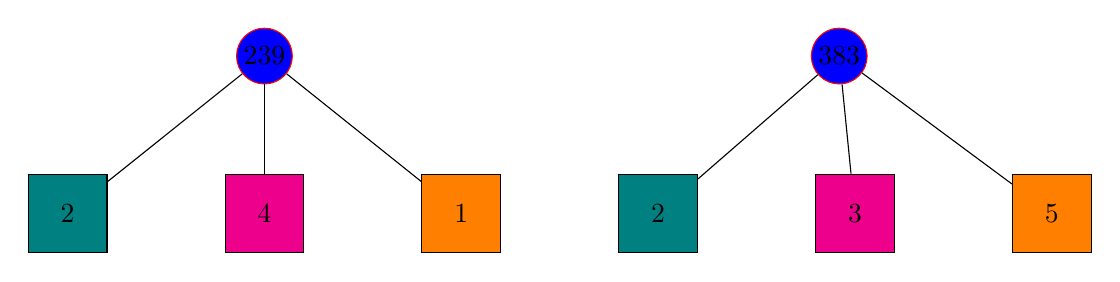
\begin{tikzpicture}
\tikzstyle{point2}=[circle, draw=red, fill=blue, inner sep=0.05cm]
    \node[rectangle,draw, fill=teal, minimum width = 1cm,
    minimum height = 1cm] (r1) at (0,0) {$2$};
 \node[rectangle,draw,  fill= magenta, minimum width = 1cm,
    minimum height = 1cm] (r2) at (2.5,0) {$4$};
 \node[rectangle,draw, fill= orange, minimum width = 1cm,
    minimum height = 1cm] (r3) at (5,0) {$1$};

    \node[rectangle,draw, fill=teal, minimum width = 1cm,
    minimum height = 1cm] (q1) at (7.5,0) {$2$};
 \node[rectangle,draw,  fill=magenta, minimum width = 1cm,
    minimum height = 1cm] (q2) at (10,0) {$3$};
 \node[rectangle,draw, fill=orange, minimum width = 1cm,
    minimum height = 1cm] (q3) at (12.5,0) {$5$};


\node (X) at (2.5,2) [point2] {$239$};
\draw (X)--(r1);
\draw (X)--(r2);
\draw (X)--(r3);

\node (Y) at (9.8,2) [point2] {$383$};
\draw (Y)--(q1);
\draw (Y)--(q2);
\draw (Y)--(q3);
\end{tikzpicture}


\end{stepitemize}

\end{frame}

\begin{frame}{Operating on Slots}
\begin{stepitemize}
    \item To calculate $239+383$ and $239\cdot 383$ modulo $105$.
    \item Just do this on slots, component-wise:

    \bigskip

        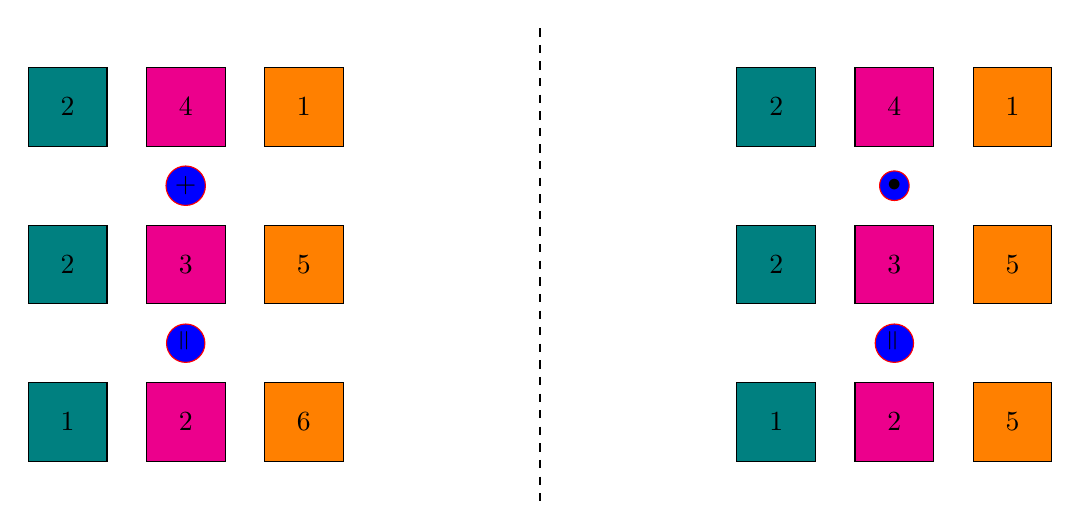
\begin{tikzpicture}
\tikzstyle{point2}=[ circle, draw=red, fill=blue, inner sep=0.05cm]

    \node[rectangle,draw, fill=teal, minimum width = 1cm,
    minimum height = 1cm] (r1) at (0,0) {$2$};
 \node[rectangle,draw,  fill= magenta, minimum width = 1cm,
    minimum height = 1cm] (r2) at (1.5,0) {$4$};
 \node[rectangle,draw, fill= orange, minimum width = 1cm,
    minimum height = 1cm] (r3) at (3,0) {$1$};

    \node[rectangle,draw, fill=teal, minimum width = 1cm,
    minimum height = 1cm] (q1) at (0,-2) {$2$};
 \node[rectangle,draw,  fill=magenta, minimum width = 1cm,
    minimum height = 1cm] (q2) at (1.5,-2) {$3$};
 \node[rectangle,draw, fill=orange, minimum width = 1cm,
    minimum height = 1cm] (q3) at (3,-2) {$5$};

    \node[rectangle,draw, fill=teal, minimum width = 1cm,
    minimum height = 1cm] (s1) at (0,-4) {$1$};
 \node[rectangle,draw,  fill=magenta, minimum width = 1cm,
    minimum height = 1cm] (s2) at (1.5,-4) {$2$};
 \node[rectangle,draw, fill=orange, minimum width = 1cm,
    minimum height = 1cm] (s3) at (3,-4) {$6$};

\node (X) at (1.5,-1) [point2] {$+$};
\node (Y) at (1.5,-3) [point2] {$\verteq$};

  \node[rectangle,draw, fill=teal, minimum width = 1cm,
    minimum height = 1cm] (t1) at (9,0) {$2$};
 \node[rectangle,draw,  fill= magenta, minimum width = 1cm,
    minimum height = 1cm] (t2) at (10.5,0) {$4$};
 \node[rectangle,draw, fill= orange, minimum width = 1cm,
    minimum height = 1cm] (t3) at (12,0) {$1$};

    \node[rectangle,draw, fill=teal, minimum width = 1cm,
    minimum height = 1cm] (u1) at (9,-2) {$2$};
 \node[rectangle,draw,  fill=magenta, minimum width = 1cm,
    minimum height = 1cm] (u2) at (10.5,-2) {$3$};
 \node[rectangle,draw, fill=orange, minimum width = 1cm,
    minimum height = 1cm] (u3) at (12,-2) {$5$};

    \node[rectangle,draw, fill=teal, minimum width = 1cm,
    minimum height = 1cm] (v1) at (9,-4) {$1$};
 \node[rectangle,draw,  fill=magenta, minimum width = 1cm,
    minimum height = 1cm] (v2) at (10.5,-4) {$2$};
 \node[rectangle,draw, fill=orange, minimum width = 1cm,
    minimum height = 1cm] (v3) at (12,-4) {$5$};

\node (Z) at (10.5,-1) [point2] {$\bullet$};
\node (W) at (10.5,-3) [point2] {$\verteq$};
\draw[dashed] (6,1) -- (6,-5);

\end{tikzpicture}
\end{stepitemize}
\end{frame}

\begin{frame}{Correctness of the results}
\begin{stepitemize}
    \item Apply the CRT algorithm to the slots we get
    \item $239+383 \equiv 97 \pmod{105} \:\:\:\: \checkmark$
    \item $239\cdot 383 \equiv 82\pmod{105} \:\:\:\: \checkmark$
\end{stepitemize}

\end{frame}
\begin{frame}{CRT and Slots for Polynomials}
\begin{stepitemize}
    \item CRT and slots work for polynomials as well.
    \item This allows for simpler operations in HE.
\end{stepitemize}
\end{frame}

\begin{frame}{Do we always have slots for polynomials?}
    \begin{stepitemize}
    \item $f(x)$, modulus polynomial, needs to be ``decomposed" into smaller, coprime factors.
    \item This always happens for integer modulus
    \item What about polynomials?
%    \item Yes if modulus polynomial is special
    \end{stepitemize}
\end{frame}

\begin{frame}{Cyclotomics}
    \begin{stepitemize}
    \item The $m$th cyclotomic polynomial $\Phi_m(x)$
    \item Degree $\phi(m)$ (Euler's Totient Function).
    \item $x^n-1 = \prod_{\ell|n}\Phi_{\ell}(x)$.
    \item $\Phi_1(x)=x-1$
    \\ $\Phi_2(x)=x+1$,
    \\ $\Phi_3(x)=x^2+x+1$, \\
    $\Phi_4(x)= x^2+1$, etc.
    \item If $p$ prime with $p^d\equiv 1\pmod{m}$ and $d$ is the smallest such integer then
    $$\Phi_m(x) = f_1(x)f_2(x) \dots f_n(x) \pmod{p}.$$
    \item Each $f_i(x)$ of degree $d$ and $n=\phi(m)/d$.
    \item $f_i(x)$ are all irreducible and coprime.
    \item When $p\equiv 1\pmod{m}$, $f_i(x)$ are linear.
    \end{stepitemize}
\end{frame}

\begin{frame}{Example of CRT for polynomials}
    \begin{stepitemize}
    \item Let $m=12$
    \item So $\Phi_{12}(x)=x^4-x^2+1$.
    \item Take $p=61$. ( $61\equiv 1\pmod{12}$.)
    \item $x^4-x^2+1 = (x+21)(x+29)(x+32)(x+40) \pmod{61}.$
    \item So we are working in $\Z_{61}[x]$.
%    \item $f(x)$ modulo lin. polynomial is easy.
    \item $f(x) \equiv f(-a) \pmod{x+a}$.
    \end{stepitemize}
\end{frame}

\begin{frame}{The Slots and operations}
  \begin{stepitemize}
\item The slots for
\begin{align*} f(x)&=x^3+23x^2-12x+2 \\
g(x)&=x^3-11x^2+x-24
\end{align*}
\item[]
  \bigskip
\begin{center}
    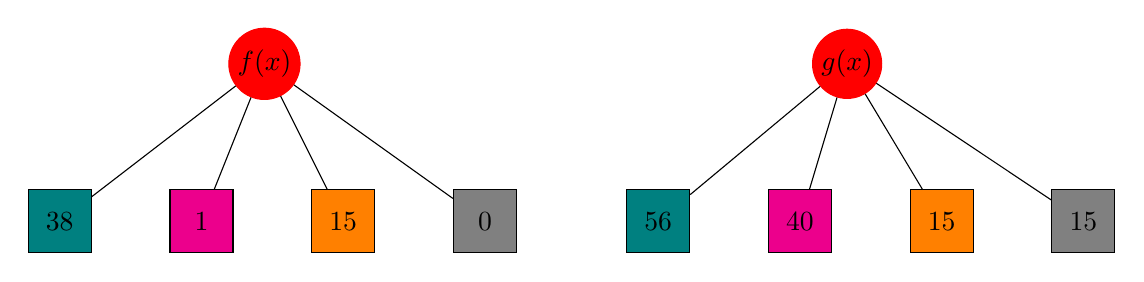
\begin{tikzpicture}
\tikzstyle{point2}=[circle, fill=red, draw=red, inner sep=0.05cm]

    \node[rectangle,draw, fill=teal, minimum width = 0.8cm,
    minimum height = 0.8cm] (r1) at (0,0) {$38$};
 \node[rectangle,draw,  fill= magenta, minimum width = 0.8cm,
    minimum height = 0.8cm] (r2) at (1.8,0) {$1$};
 \node[rectangle,draw, fill= orange, minimum width = 0.8cm,
    minimum height = 0.8cm] (r3) at (3.6,0) {$15$};
\node[rectangle,draw, fill= gray, minimum width = 0.8cm,
    minimum height = 0.8cm] (r4) at (5.4,0) {$0$};


    \node[rectangle,draw, fill=teal, minimum width = 0.8cm,
    minimum height = 0.8cm] (q1) at (7.6,0) {$56$};
 \node[rectangle,draw,  fill=magenta, minimum width = 0.8cm,
    minimum height = 0.8cm] (q2) at (9.4,0) {$40$};
 \node[rectangle,draw, fill=orange, minimum width = 0.8cm,
    minimum height = 0.8cm] (q3) at (11.2,0) {$15$};
\node[rectangle,draw, fill=gray, minimum width = 0.8cm,
    minimum height = 0.8cm] (q4) at (13,0) {$15$};


\node (X) at (2.6,2) [point2] {$f(x)$};
\draw (X)--(r1);
\draw (X)--(r2);
\draw (X)--(r3);
\draw (X)--(r4);

\node (Y) at (10,2) [point2] {$g(x)$};
\draw (Y)--(q1);
\draw (Y)--(q2);
\draw (Y)--(q3);
\draw (Y)--(q4);
\end{tikzpicture}
\end{center}
\end{stepitemize}
\end{frame}

\begin{frame}{Adding and Multiplying Polynomials}
    \begin{stepitemize}
    \item Can add and multiply $f(x)$ and $g(x)$ in $\Z_{61}[x]/(x^4-x^2+1)$.
    \item Component-wise on slots:

    \bigskip

        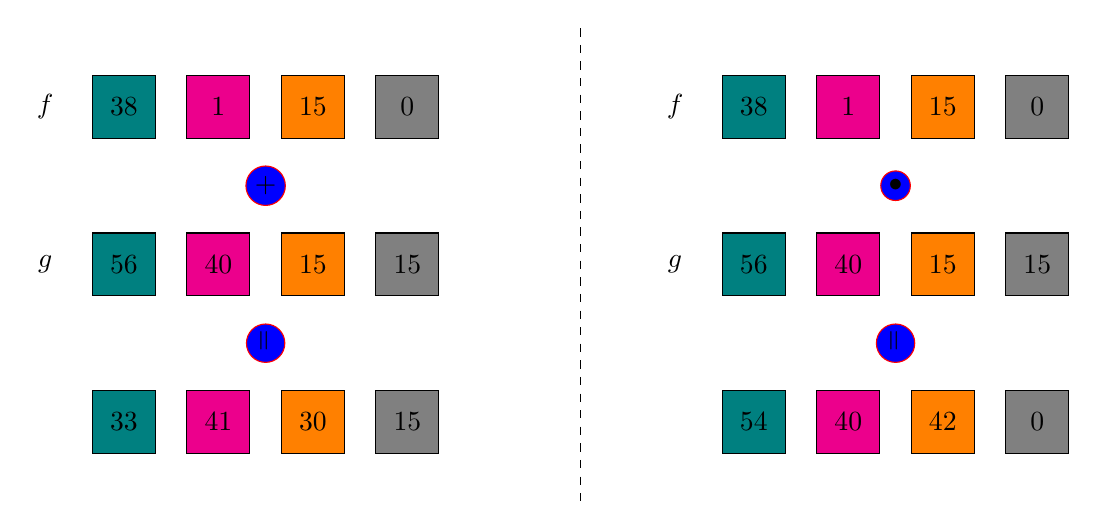
\begin{tikzpicture}
    \tikzstyle{point2}=[circle, fill=blue, draw=red, inner sep=0.05cm]
    \node[rectangle,draw, fill=teal, minimum width = 0.8cm,
    minimum height = 0.8cm] (r1) at (0,0) {$38$};
 \node[rectangle,draw,  fill= magenta, minimum width = 0.8cm,
    minimum height = 0.8cm] (r2) at (1.2,0) {$1$};
 \node[rectangle,draw, fill= orange, minimum width = 0.8cm,
    minimum height = 0.8cm] (r3) at (2.4,0) {$15$};
\node[rectangle,draw, fill= gray, minimum width = 0.8cm,
    minimum height = 0.8cm] (r4) at (3.6,0) {$0$};

        \node[rectangle,draw, fill=teal, minimum width = 0.8cm,
    minimum height = 0.8cm] (q1) at (0,-2) {$56$};
 \node[rectangle,draw,  fill=magenta, minimum width = 0.8cm,
    minimum height = 0.8cm] (q2) at (1.2,-2) {$40$};
 \node[rectangle,draw, fill=orange, minimum width = 0.8cm,
    minimum height = 0.8cm] (q3) at (2.4,-2) {$15$};
\node[rectangle,draw, fill=gray, minimum width = 0.8cm,
    minimum height = 0.8cm] (q4) at (3.6,-2) {$15$};

    \node[rectangle,draw, fill=teal, minimum width = 0.8cm,
    minimum height = 0.8cm] (s1) at (0,-4) {$33$};
 \node[rectangle,draw,  fill=magenta, minimum width = 0.8cm,
    minimum height = 0.8cm] (s2) at (1.2,-4) {$41$};
 \node[rectangle,draw, fill=orange, minimum width = 0.8cm,
    minimum height = 0.8cm] (s3) at (2.4,-4) {$30$};
\node[rectangle,draw, fill=gray, minimum width = 0.8cm,
    minimum height = 0.8cm] (s4) at (3.6,-4) {$15$};
\node (X) at (1.8,-1) [point2] {$+$};
\node (Y) at (1.8,-3) [point2] {$\verteq$};

    \node[rectangle,draw, fill=teal, minimum width = 0.8cm,
    minimum height = 0.8cm] (v1) at (8,0) {$38$};
 \node[rectangle,draw,  fill= magenta, minimum width = 0.8cm,
    minimum height = 0.8cm] (v2) at (9.2,0) {$1$};
 \node[rectangle,draw, fill= orange, minimum width = 0.8cm,
    minimum height = 0.8cm] (v3) at (10.4,0) {$15$};
\node[rectangle,draw, fill= gray, minimum width = 0.8cm,
    minimum height = 0.8cm] (v4) at (11.6,0) {$0$};

        \node[rectangle,draw, fill=teal, minimum width = 0.8cm,
    minimum height = 0.8cm] (t1) at (8,-2) {$56$};
 \node[rectangle,draw,  fill=magenta, minimum width = 0.8cm,
    minimum height = 0.8cm] (t2) at (9.2,-2) {$40$};
 \node[rectangle,draw, fill=orange, minimum width = 0.8cm,
    minimum height = 0.8cm] (t3) at (10.4,-2) {$15$};
\node[rectangle,draw, fill=gray, minimum width = 0.8cm,
    minimum height = 0.8cm] (t4) at (11.6,-2) {$15$};

    \node[rectangle,draw, fill=teal, minimum width = 0.8cm,
    minimum height = 0.8cm] (u1) at (8,-4) {$54$};
 \node[rectangle,draw,  fill=magenta, minimum width = 0.8cm,
    minimum height = 0.8cm] (u2) at (9.2,-4) {$40$};
 \node[rectangle,draw, fill=orange, minimum width = 0.8cm,
    minimum height = 0.8cm] (u3) at (10.4,-4) {$42$};
\node[rectangle,draw, fill=gray, minimum width = 0.8cm,
    minimum height = 0.8cm] (u4) at (11.6,-4) {$0$};
\node (Z) at (9.8,-1) [point2] {$\bullet$};
\node (W) at (9.8,-3) [point2] {$\verteq$};
\draw[dashed] (5.8,1) -- (5.8,-5);
\node at (-1,0) {$f$};
\node at (-1,-2) {$g$};
\node at (7,0) {$f$};
\node at (7,-2) {$g$};


\end{tikzpicture}

    \end{stepitemize}
\end{frame}

\section{LWE-RLWE Encryption, Decryption}

\begin{frame}{The LWE Problem (Oded Regev, 2005)}
\begin{stepitemize}
\item $y=x\cdot s$,
\item $x$ and $y$ known, $s$ unknown.
\item Trivial to solve.
\item But now add an error
\item $y=x\cdot s+e$
\item Hard to solve.
\item RLWE is the ring version
\item Operations done over polynomials.
\end{stepitemize}

\end{frame}

\begin{frame}{RLWE plaintext and ciphertext}
\begin{stepitemize}
\item Plaintext and ciphertext in HE from the RLWE scheme
\item $\Phi_m(x)\rightarrow $ cyclotomic,
\item $\Z_p[x]/(\Phi_m(x))\rightarrow$ plaintext space
\item $\Z_q[x]/(\Phi_m(x))\rightarrow $ ciphertext space
\item Secret key $\rightarrow$ the pair $sk=(1, \mathfrak{s})$.
\item For public key, choose polynomials $c_0^*$ and $c_1^*$ such that
$c_0^*=pe^*-c_1^*\mathfrak{s}$ and then $pk=(c_0^*, c_1^*)$.
\item To encrypt $a$,
$$E(a) = (c_0,c_1) = r(c_0^*,c_1^*)+p(e_0,e_1)+(a,0).$$
\item So
$$c_0 = rc_0^*+pe_0+a$$
$$c_1 = rc_1^*+pe_1.$$
\end{stepitemize}
\end{frame}

\begin{frame}{Decryption}
    \begin{stepitemize}
    \item To decrypt, inner product the ciphertext with the secret key,
    \item So $\langle (c_0,c_1),(1, \mathfrak{s})\rangle = c_0+c_1\mathfrak{s} = p(re^*+e_0+\mathfrak{s}e_1)+a$
    \item This is $a$ modulo $p$.
    \end{stepitemize}
\end{frame}

\begin{frame}{Addition}
    \begin{stepitemize}
    \item Two ciphertexts $E(a)$ and $E(b)$ corresponding to plaintexts $a$ and $b$:
    \item $E(a) = (c_{0,a},c_{1,a}) = r_a(c_0^*,c_1^*)+p(e_{0,a},e_{1,a})+({\color{cyan}a},0).$
    \item $E(b) = (c_{0,b},c_{1,b}) = r_b(c_0^*,c_1^*)+p(e_{0,b},e_{1,b})+({\color{magenta}b},0).$
    \item Then we have
    $$E(a)+E(b) = (r_a+r_b)(c_0^*, c_1^*)+p(e_{0,a}+e_{0,b}, e_{1,a}+e_{1,b})+({\color{cyan}a}+{\color{magenta}b},0).$$
    \item Take the inner product with $(1,\mathfrak{s})$:
    \begin{align*}
        \langle E(a)+E(b), (1, \mathfrak{s})\rangle &= p[(r_a+r_b)e^*+e_{0,a}+e_{0,b}+\mathfrak{s}(e_{1,a}+e_{1,b})]+{\color{cyan}a}+{\color{magenta}b}.
    \end{align*}

    \end{stepitemize}
\end{frame}

\section{A Basic Example}

\begin{frame}{Key Value Database}
    %\begin{stepitemize}
    %\item Privacy preserving database look up.
    %\item For example: countries and capitals
    %\item $(k,v)$-database where the keys $k$ are unique.
    %\item[]
    %\begin{center}
    %\includegraphics[scale=.38]{KV-1.jpg}
%\end{center}
 %   \end{stepitemize}

\begin{center}
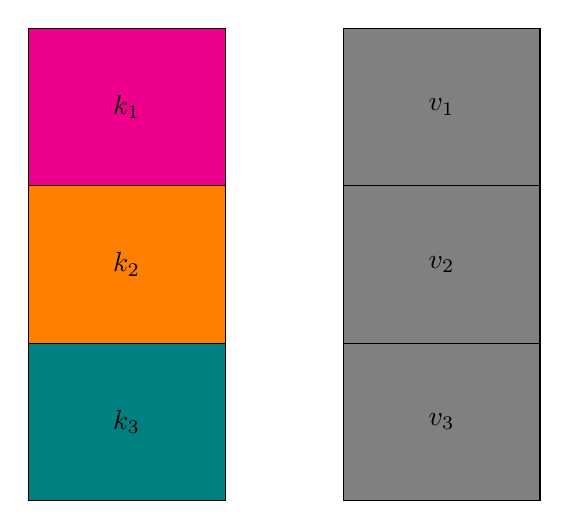
\begin{tikzpicture}
\node[rectangle,draw, fill=magenta, minimum width = 2.5cm,
    minimum height = 2cm] (r1) at (0,0) {$k_1$};
 \node[rectangle,draw,  fill= orange, minimum width = 2.5cm,
    minimum height = 2cm] (r2) at (0,-2) {$k_2$};
 \node[rectangle,draw, fill= teal, minimum width = 2.5cm,
    minimum height = 2cm] (r3) at (0,-4) {$k_3$};

\node[rectangle,draw, fill=gray, minimum width = 2.5cm,
    minimum height = 2cm] (r1) at (4,0) {$v_1$};
 \node[rectangle,draw,  fill= gray, minimum width = 2.5cm,
    minimum height = 2cm] (r2) at (4,-2) {$v_2$};
 \node[rectangle,draw, fill= gray, minimum width = 2.5cm,
    minimum height = 2cm] (r3) at (4,-4) {$v_3$};
\end{tikzpicture}
\end{center}

\end{frame}

\begin{frame}{Secure Query}
%\begin{stepitemize}
%\item Fora query $k_q$, want to securely compare it with each $k_i$
%\item Ideally want a mask with $1\rightarrow $ match, $0\rightarrow$ no match.
%\item will work nicely since keys are unique.
%\item[]
%\begin{center}
 %   \includegraphics[scale=.35]{KV-2.jpg}
%\end{center}
%\end{stepitemize}

\begin{center}
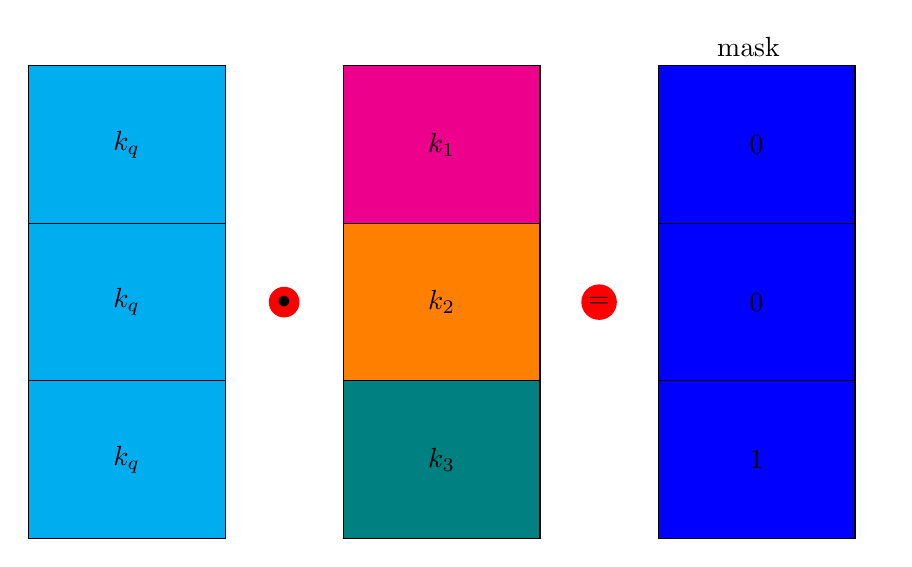
\begin{tikzpicture}
\node[rectangle,draw, fill=cyan, minimum width = 2.5cm,
    minimum height = 2cm] (r1) at (0,0) {$k_q$};
 \node[rectangle,draw,  fill= cyan, minimum width = 2.5cm,
    minimum height = 2cm] (r2) at (0,-2) {$k_q$};
 \node[rectangle,draw, fill= cyan, minimum width = 2.5cm,
    minimum height = 2cm] (r3) at (0,-4) {$k_q$};

\node[rectangle,draw, fill=magenta, minimum width = 2.5cm,
    minimum height = 2cm] (r1) at (4,0) {$k_1$};
 \node[rectangle,draw,  fill= orange, minimum width = 2.5cm,
    minimum height = 2cm] (r2) at (4,-2) {$k_2$};
 \node[rectangle,draw, fill= teal, minimum width = 2.5cm,
    minimum height = 2cm] (r3) at (4,-4) {$k_3$};

\node[rectangle,draw, fill=blue, minimum width = 2.5cm,
    minimum height = 2cm] (r1) at (8,0) {$0$};
 \node[rectangle,draw,  fill= blue, minimum width = 2.5cm,
    minimum height = 2cm] (r2) at (8,-2) {$0$};
 \node[rectangle,draw, fill= blue, minimum width = 2.5cm,
    minimum height = 2cm] (r3) at (8,-4) {$1$};

\node [above, text width=2 cm] at (8.5,1) {mask};
\tikzstyle{point2}=[circle, fill=red, draw=red, inner sep=0.05cm]

\node (X) at (2,-2) [point2] {$\bullet$};
\node (Y) at (6,-2) [point2] {$=$};
\end{tikzpicture}
\end{center}

\end{frame}

\begin{frame}{Key-Value Extraction}
   % \begin{stepitemize}
   % \item If we had the mask, just multiply across the values of the database entry-wise.

   % \bigskip
    %\item[]
%\begin{center}
 %   \includegraphics[scale=.38]{KV-3.jpg}
%\end{center}
 %\end{stepitemize}

\begin{center}
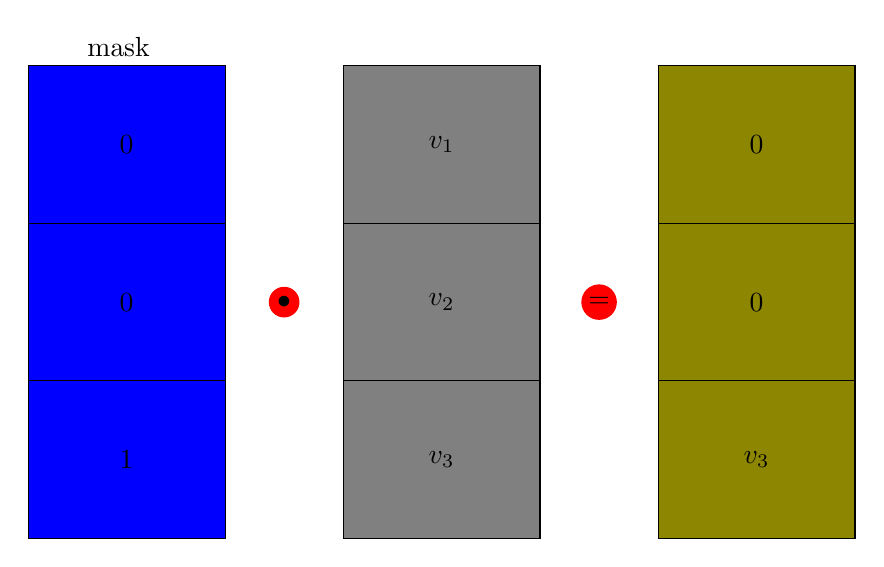
\begin{tikzpicture}
\node[rectangle,draw, fill=blue, minimum width = 2.5cm,
    minimum height = 2cm] (r1) at (0,0) {$0$};
 \node[rectangle,draw,  fill= blue, minimum width = 2.5cm,
    minimum height = 2cm] (r2) at (0,-2) {$0$};
 \node[rectangle,draw, fill= blue, minimum width = 2.5cm,
    minimum height = 2cm] (r3) at (0,-4) {$1$};

\node[rectangle,draw, fill=gray, minimum width = 2.5cm,
    minimum height = 2cm] (r1) at (4,0) {$v_1$};
 \node[rectangle,draw,  fill= gray, minimum width = 2.5cm,
    minimum height = 2cm] (r2) at (4,-2) {$v_2$};
 \node[rectangle,draw, fill= gray, minimum width = 2.5cm,
    minimum height = 2cm] (r3) at (4,-4) {$v_3$};

\node[rectangle,draw, fill=olive, minimum width = 2.5cm,
    minimum height = 2cm] (r1) at (8,0) {$0$};
 \node[rectangle,draw,  fill= olive, minimum width = 2.5cm,
    minimum height = 2cm] (r2) at (8,-2) {$0$};
 \node[rectangle,draw, fill= olive, minimum width = 2.5cm,
    minimum height = 2cm] (r3) at (8,-4) {$v_3$};

\node [above, text width=2 cm] at (0.5,1) {mask};
\tikzstyle{point2}=[circle, fill=red, draw=red, inner sep=0.05cm]

\node (X) at (2,-2) [point2] {$\bullet$};
\node (Y) at (6,-2) [point2] {$=$};
\end{tikzpicture}
\end{center}


\end{frame}
\begin{frame}{The Difference Operator}
%\begin{stepitemize}
%\item So how do we homomorphically get such a mask?
 %   \item First, calculate differences
  %  \item $0\rightarrow$ match, a non-zero value otherwise.
   %
   % \bigskip
   % \item[]
   % \begin{center}
   % \includegraphics[scale=.38]{KV-4.jpg}
%\end{center}
%\end{stepitemize}

\begin{center}
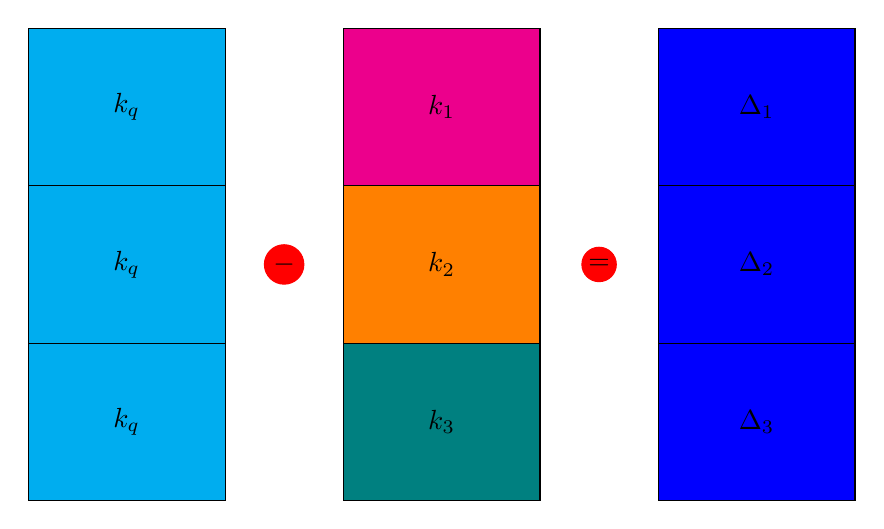
\begin{tikzpicture}
\node[rectangle,draw, fill=cyan, minimum width = 2.5cm,
    minimum height = 2cm] (r1) at (0,0) {$k_q$};
 \node[rectangle,draw,  fill= cyan, minimum width = 2.5cm,
    minimum height = 2cm] (r2) at (0,-2) {$k_q$};
 \node[rectangle,draw, fill= cyan, minimum width = 2.5cm,
    minimum height = 2cm] (r3) at (0,-4) {$k_q$};

\node[rectangle,draw, fill=magenta, minimum width = 2.5cm,
    minimum height = 2cm] (r1) at (4,0) {$k_1$};
 \node[rectangle,draw,  fill= orange, minimum width = 2.5cm,
    minimum height = 2cm] (r2) at (4,-2) {$k_2$};
 \node[rectangle,draw, fill= teal, minimum width = 2.5cm,
    minimum height = 2cm] (r3) at (4,-4) {$k_3$};

\node[rectangle,draw, fill=blue, minimum width = 2.5cm,
    minimum height = 2cm] (r1) at (8,0) {$\Delta_1$};
 \node[rectangle,draw,  fill= blue, minimum width = 2.5cm,
    minimum height = 2cm] (r2) at (8,-2) {$\Delta_2$};
 \node[rectangle,draw, fill= blue, minimum width = 2.5cm,
    minimum height = 2cm] (r3) at (8,-4) {$\Delta_3$};

\tikzstyle{point2}=[circle, fill=red, draw=red, inner sep=0.05cm]

\node (X) at (2,-2) [point2] {$-$};
\node (Y) at (6,-2) [point2] {$=$};
\end{tikzpicture}
\end{center}

\end{frame}
\begin{frame}{Fermat's Little Theorem}
\begin{stepitemize}
\item If $p$ is prime and $a$ is any integer, then
$$ a^{p-1}\equiv    \left \{ \begin{array}{ll}
1 \pmod{p} & \textrm{if $p\nmid a$ }\\
0 \pmod{p} & \textrm {if $p | a$}
\end{array}\right.$$
\item Denote by $FLT(x)$ and since we are in $\Z_p$:
$$ FLT(x) = \left \{ \begin{array}{ll}
1  & \textrm{if $x\neq 0$ }\\
0 & \textrm {if $x=0$}
\end{array}\right.$$
\item Take the complement:
$$1-FLT(x) = \left \{ \begin{array}{ll}
0  & \textrm{if $x\neq 0$ }\\
1 & \textrm {if $x=0$}
\end{array}\right.$$
\end{stepitemize}
\end{frame}

\begin{frame}{Key-Value $1-$FLT}
    %\begin{stepitemize}
    %\item So applying $1$-FLT will do the job:
    %\bigskip
    %\item[]
    %\begin{center}
    %\includegraphics[scale=.38]{KV-6.jpg}
%\end{center}
%\end{stepitemize}

\begin{center}
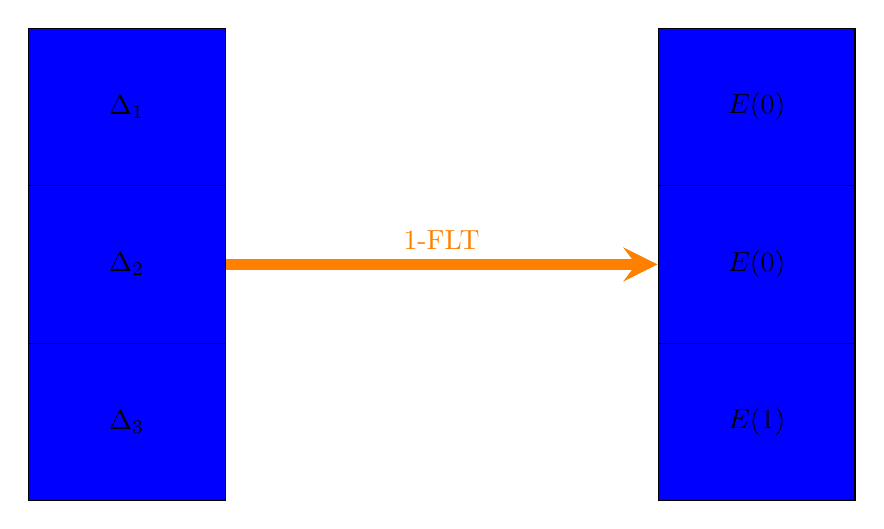
\begin{tikzpicture}
\node[rectangle,draw, fill=blue, minimum width = 2.5cm,
    minimum height = 2cm] (r1) at (0,0) {$\Delta_1$};
 \node[rectangle,draw,  fill= blue, minimum width = 2.5cm,
    minimum height = 2cm] (r2) at (0,-2) {$\Delta_2$};
 \node[rectangle,draw, fill= blue, minimum width = 2.5cm,
    minimum height = 2cm] (r3) at (0,-4) {$\Delta_3$};

\node[rectangle,draw, fill=blue, minimum width = 2.5cm,
    minimum height = 2cm] (q1) at (8,0) {$E(0)$};
 \node[rectangle,draw,  fill= blue, minimum width = 2.5cm,
    minimum height = 2cm] (q2) at (8,-2) {$E(0)$};
 \node[rectangle,draw, fill= blue, minimum width = 2.5cm,
    minimum height = 2cm] (q3) at (8,-4) {$E(1)$};

\draw[-stealth, color=orange, line width=1.5mm] (r2)--node [above] {1-FLT}(q2);
\end{tikzpicture}
\end{center}
\end{frame}

\begin{frame}{Key-Value Extraction}
%\begin{stepitemize}
 %   \item Multiply the mask with the values
  %  \bigskip
  % \item []
    % \begin{center}
%    \includegraphics[scale=.38]{KV-7.jpg}
%\end{center}
%\end{stepitemize}
 \begin{center}
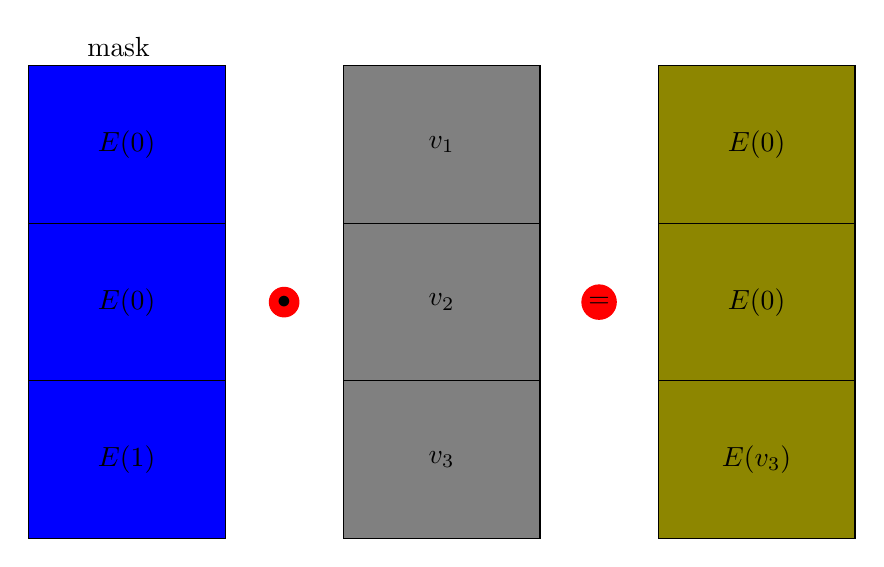
\begin{tikzpicture}
\node[rectangle,draw, fill=blue, minimum width = 2.5cm,
    minimum height = 2cm] (r1) at (0,0) {$E(0)$};
 \node[rectangle,draw,  fill= blue, minimum width = 2.5cm,
    minimum height = 2cm] (r2) at (0,-2) {$E(0)$};
 \node[rectangle,draw, fill= blue, minimum width = 2.5cm,
    minimum height = 2cm] (r3) at (0,-4) {$E(1)$};

\node[rectangle,draw, fill=gray, minimum width = 2.5cm,
    minimum height = 2cm] (r1) at (4,0) {$v_1$};
 \node[rectangle,draw,  fill= gray, minimum width = 2.5cm,
    minimum height = 2cm] (r2) at (4,-2) {$v_2$};
 \node[rectangle,draw, fill= gray, minimum width = 2.5cm,
    minimum height = 2cm] (r3) at (4,-4) {$v_3$};

\node[rectangle,draw, fill=olive, minimum width = 2.5cm,
    minimum height = 2cm] (r1) at (8,0) {$E(0)$};
 \node[rectangle,draw,  fill= olive, minimum width = 2.5cm,
    minimum height = 2cm] (r2) at (8,-2) {$E(0)$};
 \node[rectangle,draw, fill= olive, minimum width = 2.5cm,
    minimum height = 2cm] (r3) at (8,-4) {$E(v_3)$};

\node [above, text width=2 cm] at (0.5,1) {mask};
\tikzstyle{point2}=[circle, fill=red, draw=red, inner sep=0.05cm]

\node (X) at (2,-2) [point2] {$\bullet$};
\node (Y) at (6,-2) [point2] {$=$};
\end{tikzpicture}
\end{center}

\end{frame}
\begin{frame}{Key-value aggregation}
%\begin{stepitemize}
 %   \item Keys unique, at most one match per query.
  % \item So aggregate all into a single ciphertext.
   %
   % \item []
%     \begin{center}
 %   \includegraphics[scale=.38]{KV-8.jpg}
%\end{center}
%\end{stepitemize}
\begin{center}
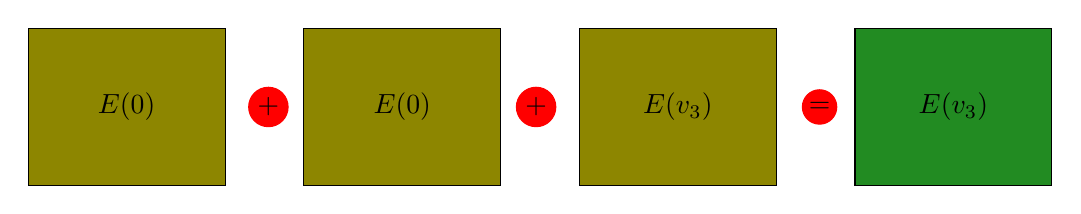
\begin{tikzpicture}
\node[rectangle,draw, fill=olive, minimum width = 2.5cm,
    minimum height = 2cm] (r1) at (0,0) {$E(0)$};
\node[rectangle,draw, fill=olive, minimum width = 2.5cm,
    minimum height = 2cm] (r1) at (3.5,0) {$E(0)$};
 \node[rectangle,draw,  fill= olive, minimum width = 2.5cm,
    minimum height = 2cm] (r2) at (7,0) {$E(v_3)$};
 \node[rectangle,draw, fill= ForestGreen, minimum width = 2.5cm,
    minimum height = 2cm] (r3) at (10.5,0) {$E(v_3)$};

\tikzstyle{point2}=[circle, fill=red, draw=red, inner sep=0.05cm]

\node (X) at (1.8,0) [point2] {$+$};
\node (X) at (5.2,0) [point2] {$+$};
\node (Y) at (8.8,0) [point2] {$=$};
\end{tikzpicture}
\end{center}
\end{frame}

\begin{frame}
\centerline{ \bf{\large THANK YOU!!!}}

\end{frame}

\end{document}
